% This is a thesis template that attempts to conform to the guidelines
% published by UTRGV's Graduate School office.

% Please report any issues to
% https://github.com/UTRGV-SMSS/Thesis-Template/issues

% The author of this template is Guillermo Garza.


% Switch this line to the final option when submitting your thesis.
% This will correct counts and remove labels that are shown during draft mode
%\documentclass[masters,draft]{UTRGVthesis}
\documentclass[masters,final]{UTRGVthesis}
%\documentclass[phd,draft]{UTRGVthesis}
%\documentclass[masters,final, nodedication, noacknowledgments]{UTRGVthesis}


% Load your packages below.
% Make hyperref and showkeys come at the end of your loaded packages
% to make sure they are not over-written.  They redefine many
% standard LaTeX commands
\usepackage{docmute} % for inputting complete documents. Useful for LyX users
\usepackage{booktabs} % for better tables
\usepackage{microtype} % for better typography
\usepackage[colorlinks=false]{hyperref}  % for urls
\usepackage{showkeys} % shows labels during draft mode
\usepackage{xfrac}
\usepackage{multirow}
%\usepackage[document]{ragged2e} % uncomment for non-justified text


% Uncomment the line below to check if text is aligned to margins
%\margins

% To change body font from Times Roman to Times New Roman, compile with XeLaTeX
% This assumes you have Times New Roman font installed in your machine
% WARNING! This will NOT change the font in Math Environments
\usepackage{ifxetex}
\ifxetex
   \usepackage{fontspec}
   \setmainfont{Times New Roman}
\fi

% this sets the name of the bibliography
% add \vspace{1cm} here to adjust vertical spacing after bibliography title
\renewcommand{\bibname}{BIBLIOGRAPHY}


% Insert your name and major here in the format shown
\Author{Suryarao Bethapudi}
\AuthorLastFirst{Bethapudi, Suryarao}
\Major{Physics}


% Insert your graduation date here
\Month{August}
\Year{2020}


% Insert the title of your thesis here.
% If you have a long title, split it between multiple lines using the \\ command
% Also, use comment characters to avoid unwanted spaces in the Abstract page
\Title{Searching for low frequency Fast Radio Bursts with\\
	VLITE
}


% Insert your research advisor and his title here
\Advisor{Dr. Teviet Creighton}
\AdvisorTitle{Chair of Committee}


% Insert the members of your committee here
% You can also give MemberA a special title
\MemberA{Dr. Volker Questchke}  %\MemberATitle{Co-Chair of Committee}
\MemberB{Dr. Soumya Mohanty}  %\MemberATitle{Co-Chair of Committee}
%\MemberB{Dr. Soma Mukherjee}  %\MemberBTitle{Co-Chair of Committee}
%\MemberC{}
%\MemberD{}
%\MemberE{}


% Insert the text of your abstract below.
% The bibliography style "citation" required by the manual is automatically
% generated.  Specify the "final" option in the \documentclass to update the
% counts to the correct values.
\Abstract{%
	The VLITE (VLA Low Band Ionosphere and Transient Experiment; http://vlite.nrao.edu) program performs commensal observations using 16 antennas of the Very Large Array radio telescope from 320-384 MHz. The VLITE-Fast program searches for short time-scale (<100ms) transients, such as Fast Radio Bursts (FRBs), in real time and triggers recording of baseband voltages for offline imaging. Searches are made possible by a 12 node cluster, each housing GPUs for digital signal processing. A real-time Message Passing Interface (MPI)-based co-adder incoherently sums the data streams from all the antennas to boost the signal-to-noise. To undo the dispersion effects of signal propagation through the ionized interstellar medium, the co-added stream is de-dispersed and matched-filtered to search for transients. This operation is completely performed on GPUs by the software package Heimdall . A selection logic is applied to the candidates and interesting candidates with their corresponding data are processed and packaged in a binary file along with a diagnostic plot. Furthermore, a Machine Learning classification is developed and applied on the reduced data product and, based on its decision, baseband voltages are recorded.  Reduced data products collected over 126 days of on-sky operation form the VLITE-Fast Pathfinder Survey (VFPS). This pipeline has triggered on single pulses from 7 known radio pulsars. Lastly, the pipeline capabilities are tested against pure random noise and simulated injected signals. 
}


% You can dedicate your paper here.  This is optional.
\Dedication{%
	\begin{center}
		\begin{emph}
			For the dreading drag until death liberates us.
		\end{emph}
	\end{center}
}


% Acknowledge those who helped and supported you here. This is optional.
\Acknowledgments{%
	I acknowledge the \ldots
}


% Insert your biographical sketch here.
\BiographicalSketch{%
	no
}

% Graphics path
\graphicspath{{figures/}}

% bibliography
\bibliography{bibs/allbibs.bib}


\begin{document}

% This starts page counting in Roman numerals
\frontmatter


% This command makes the formal preliminary pages.
% You can comment it out during the drafting process if you want to save paper.
\makepreliminarypages


% These insert a table of contents, list of tables, and list of figures
\tableofcontents
\listoftables
\listoffigures


% This starts regular page counting in Arabic numerals
\mainmatter

% This starts double-spaced text.  Opposite command is \singlespacing
\doublespacing

% custom commands
\newcommand{\vf}{\texttt{VLITE-Fast}~}
\newcommand{\dada}{\texttt{DADA}~}
\newcommand{\frb}[1]{\texttt{FRB#1}}
\newcommand{\mpi}{\texttt{mpi}~}
\newcommand{\dm}{\texttt{DM}{}}
\newcommand{\fbson}{\texttt{fbson}{}}
\newcommand{\dbson}{\texttt{dbson}{}}
\newcommand{\meta}{\texttt{meta}{}}
\newcommand{\uchar}{\texttt{uint8}{}}
\newcommand{\cc}{\emph{C}}
\newcommand{\sn}{S/N{}}
%\newcommand{\vbt}[1]{\texttt{#1}}

% OK. Everything is set up. Insert your thesis below.
% It's a good idea to split your thesis up into different files and use
% the \input command

% FRBs
\chapter{Fast Radio Bursts}\label{ch:frb}

\par The domain of Radio Astronomy is full of surprises. 
What started off as an experiment to communicate across the Atlantic ocean using radio waves soon took turn when Karl Jansky recorded radio signals emanating from the direction of our galaxy's center and established the idea of using radio telescopes to \emph{look} at the heavens.
Many decades later, the same radio astronomy discovered a new type of stars which shines but in radio regime and also pulsates like a light house. These were characterized to be pulsating source of radiation and were aptly named as pulsars.
Half a century later during which thousands of pulsars were discovered and documented, a new type of a signal emerged.
It was a serendiptious detection of \emph{a bright millisecond radio burst}~\cite{lorimerburst} in the archieval data which brought into light, the existence of short time-scale, extremely energetic radio signals, possibly originating from beyond the galaxy. 
These signals are called \emph{Fast Radio Bursts (\frb{})} and the search for these signals forms the crux of this thesis.

\par The first discovered \frb is the~\cite{lorimerburst} in $2007$, colloquially known as the \emph{Lorimer Burst} (see~\autoref{fig:lorimer}). 
Many theory papers followed but there was no corroborative detection. In the lack of which, skeptisim arose~\cite{burke_doubt}. 
Prior to that~\cite{old_m87_bursts} detected \frb-like pulses with \dm~as high as $5\times 10^3$ \pc originating from \textt{M87}. So, these may very well have been the first detection of \frb s but due to the limited time/frequency resolution, no substantiative evidence could be established. 

\begin{figure}
	\centering
	\label{fig:lorimer}
	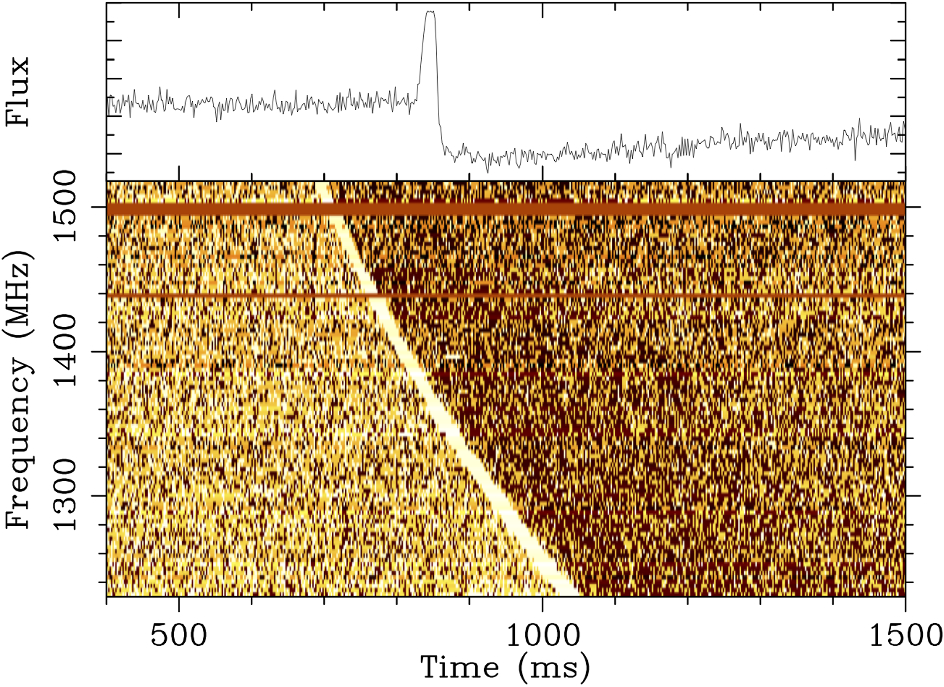
\includegraphics[width=\textwidth,keepaspectratio]{lorimer_burst.png}
	\caption{Lorimer burst. The first ever \frb{} detected. The curve in the filterbank (see~\autoref{ssub:fb}) is due to a propagation effect called dispersion (see~\autoref{ssub:dis}). The sheer strength of the signal is self evident when looking at the amplitude of the peak.}
\end{figure}

\par Astronomers were not wrong in their dubious nature. Their experience with another species of signals called Perytons~\cite{perytons} justifies it. Named after the mystical hybrid bird, these signals were actually caused by the microwave on the observatory site. The premature opening of the microwave door shuts off the magnetron abruptly, which produces a dispersed-like signal which was then picked up by the radio telescope.
This put more shade on the celestial nature of the \emph{Lorimer Burst}.

\par But then came as a surprise, ~\cite{danburst4} in $2016$, almost a decade later, which reported $4$ such bursts and thus set in stone the existence of such species. The hunt was on.
Now, four years and many sophisticated advancements in observatory technologies later, the number of \frb{}s detected is in hundreds. The details of this story will be discussed in \autoref{sec:detect_so_far}.

\par Given the amount of shear energy emitted in these bursts, astronomers were not wrong in maintaining an innate assumption that these events were result of a cataclysmic event. And by the very nature of such events, \frb{}s were not expected to repeat. And then came as a surprise, \frb{121102} in $2012$, which repeated in time.
Over the years since its discovery, \frb{121102} is perhaps the most studied \frb{} with observations done from meter wavelength to milli-meter wavelength. See~\cite{spitler, palfa_frb}.

\par Astronomy wouldn't be full of surprises, if \frb{121102}~ was the only repeating \frb{}~ found. In $2019$,~\cite{chime_repeater8,chime_repeater9} found $4$ repeating \frb{}s (henceforth called repeaters) using the Canadian Hydrogen Intensity Mapping Experiment (CHIME) telescope which prompted a fresh set of theories to emerge to explain the same.

\par All the discovered \frb{}s are catalogued in \textt{FRBCAT}~\cite{frbcat}. All the theories of \frb{}s are also catalogued in \textt{FRB-theorycat}~\cite{frbtheorycat}.


\section{What are FRBs?}

\par Before we go into \frb{}s, it is crucial to establish certain groundwork known in a radio astronomy setting. 
First being the data representation format widely used: filterbank in~\autoref{ssub:fb}. 
Second being the phenomenon of dispersion which affects all the radio signals propagating through the space and reaching the radio telescope. 
This will be covered in detail in~\autoref{sssub:dd}. 
Then, in~\autoref{ssub:dis}, \frb{}s are characterized.

\subsection{Filterbank}
\label{ssub:fb}

\par A popular data representation format for radio astronomers is the time frequency bins, known as filterbank, where every bin has one or more of the four Stokes parameter. In a typical setting, of the four, only the Stokes I is recorded.
Any radio astronomy setup involves a frequency band $[\nu_{\rm LOW}, \nu_{\rm HIGH}]$ of interest discretized into \texttt{NCHAN} frequency channels, yielding frequency channel width, denoted by \texttt{FOFF}, as bandwidth divided by the number of channels.
Time samples are sampled at a suitable Nyquist Sampling rate commensurate with the bandwidth $\nu_{\rm HIGH} - \nu_{\rm LOW}$. Let the sampling rate be \texttt{TSAMP}.

\par With the above definitions in place, starting off with voltage samples, by applying Short Time Fourier Transform and consequently taking magnitude (essentially Stokes I), filterbank is produced. In practise, a suitable digitization scheme is employed and data is digitized to \textt{NBIT} bits per sample.
Every consecutive time sample is separated by \texttt{TSAMP} in time and every consecutive frequency sample is separated by \texttt{FOFF}.
This representation makes it easier to look at the time frequency variations and hence is popular.

\subsection{Dispersion}
\label{ssub:dis}

\par Imagine sending sunlight through a prism. It is common knowledge to expect rainbow emanating from the prism. 
This same phenomenon is what brings a rainbow after the rain if the Sun is up. The physics behind this as follows:
White light is made up of the seven colors. And, when white light goes through the prism, distinct color components get separated,
and a rainbow is observed. 
This phenomenon is called dispersion and is not just valid for white light (or, visible band of electromagnetic spectrum). 
Of course, the properties of the prism changes when going to a different band of electromagnetic spectrum. But, any part of the electromagnetic spectrum can get dispersed and its frequency components can get separated. And since different frequencies of visible light correspond to different colors, we see colors of a rainbow.

\par Radio waves propagating in space also suffer the same fate. \emph{Prisms} here are plasma made of electrons in the space. 
This plasma exists in the line of sight between the source and the observatory. A better understanding of the dispersion can be made by using the filterbank representation. Dispersion causes progressively lower frequencies to receive the signal latter than their higher frequency counterpart. See fig.

\par The time difference (also known as dispersion smearing) is calculated with the~\autoref{eq:dispersion}. The \dm~appearing in the equation is called the Dispersion Measure which is a measure of the electron number density in the column along the line of sight.
\begin{equation}
\label{eq:dispersion}
\Delta t = {\rm DM} \times 4.15 \times 10^{-3} \big[  \frac{1}{\nu^2_{\rm LOW}} - \frac{1}{\nu^2_{\rm HIGH}} \big]\ {\rm s}
\end{equation}
This effect of dispersion is to be corrected for any analysis and the process is called de-dispersion. More details about de-dispersion will be covered in~\autoref{ch:inst}.

\par Dispersion is purely a propagation effect. Thus, amount of dispersion provides a good marker of distance. There are two models for electron distribution in the galaxy, NE2001~\cite{ne2001} and YMW~\cite{ymw16}. With the help of a model, given a pointing in Galactic coordinates ($l$, $b$), the \dm~contribution by the Galaxy can be estimated. This model becomes useful later when talking about \frb{} origin in following sections. 

\subsubsection {De-dispersion}
\label{sssub:dd}

\par In order to compensate for the dispersion effect, de-dispersion is performed. The de-dispersion is a computationally intensive process.
\par With a filterbank, de-dispersion can be straightforward where frequency channels are time-shifted can do the job. 
However, this does not negate dispersion effects in the frequency channel, leading to what is called the in-channel smearing.
Mathematically, it can be derived by using small bandwidth approximation to~\autoref{eq:dispersion}. 
See~\autoref{eq:inchannel} where $\Delta \nu$ is the channel bandwidth and $\nu$ is the frequency of the top end of the channel.
\begin{equation}
\label{eq:inchannel}
\Delta \tau = {\rm DM} \times 4.15 \times 10^{-3} \big[  \frac{\Delta \nu}{\nu^3}  \big]\ {\rm s}
\end{equation}

\subsection{Characteristics}
\label{ssub:frb}

\par \frb s are short time-scale ($\sim$ ms), bright ($0.001 - 100$ Jy), broadband (present in \emph{almost} all frequency channels) and extremely dispersed (very large \dm) radio signals. 
The most distinctive feature of an \frb{}~ is its \dm which is many fold more than the galaxy could contribute. The galaxy contribution to a signal detected at an observatory is calculated using the pointing information (at the time of detection) and using an eletron density model as discussed in~\autoref{sssub:dd}.

\par To further appreciate the high \dm of \frb{}~, the \dm and $\frac{\rm DM}{{\rm DM}_{\rm Max}}$ are plotted. DM$_{\rm Max}$ is maximum galactic contribution for the given pointing. See ~\autoref{fig:dmdmax} also~\cite{petroff_survey, palfa_frb}. Clearly, all the \frb{}s are atleast multiple times the galactic contribution. This inference, combined with the understanding that \dm~ is a proxy for distance, provides evidence that \frb{}s origin from extra-galactic and of cosmological nature.

\begin{figure}
\label{fig:dmdmax}
	\centering
	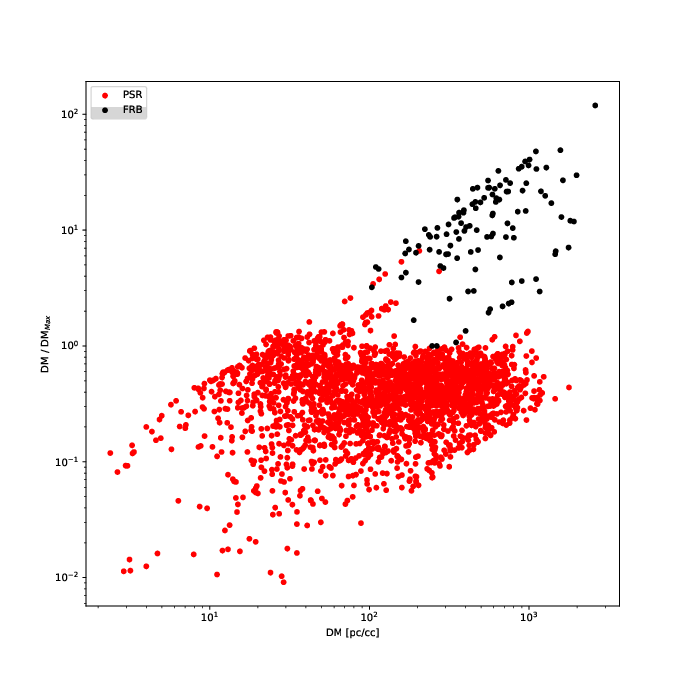
\includegraphics[width=0.8\textwidth, keepaspectratio]{dm_dmax.png}
\caption{\dm v/s $\frac{\rm DM}{{\rm DM}_{\rm Max}}$. An updated version of~\cite{petroff_survey, palfa_frb}.}
\end{figure}

\par \frb{}s also exhibit other features such as scintillation and scattering. Scintillation is the twinkling of stars phenomena one can observe. 
Scintillation presents itself in \frb{}s as the pulse disappearing for some frequency channels and appearing back when looking at the filterbank. This can be observed in the~\autoref{fig:frbset}. 
Scattering is the broadening of the pulse in the filterbank. This is also seen as an exponential tail in the frequency averaged profile.
Also see~\autoref{fig:frbset}.

\begin{figure}
	\label{fig:frbset}
	\centering
	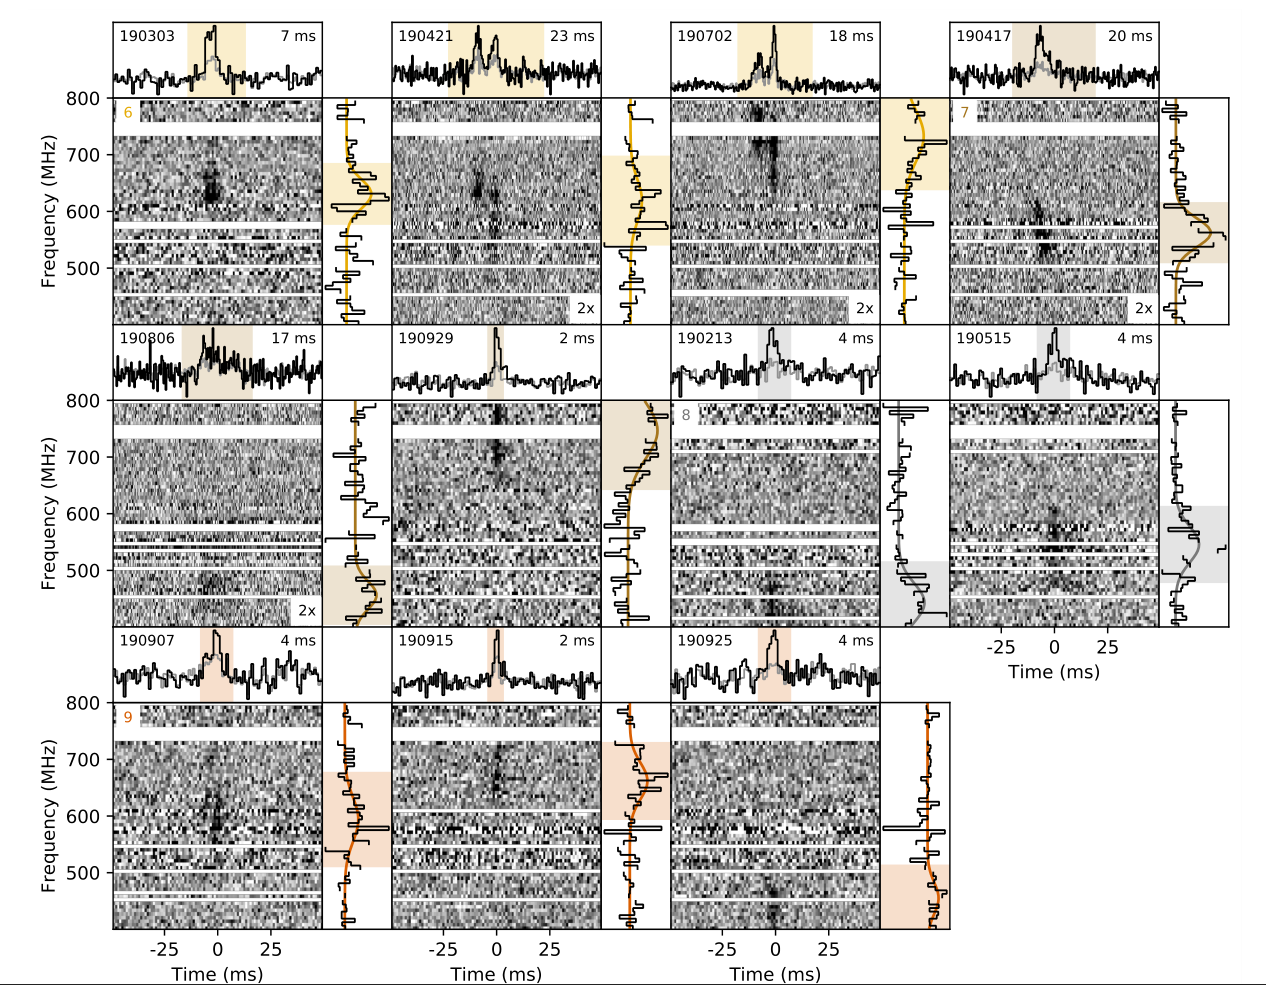
\includegraphics[width=0.8\textwidth, keepaspectratio]{frbset.png}
	\caption{A set of repeating \frb{}s detected~\cite{chime_repeater9}. Scattering causes the broadening of the pulse.}
\end{figure}

\section{Detections so far}
\label{sec:detect_so_far}

\par Using the catalogued \frb{}s from \textt{FRBCAT} mentioned before, a brief summary of the \frb{}s population is given.
Firstly, \autoref{fig:frbtime} summarizes the \frb{}s detected by various instruments over time. \autoref{fig:frbsky} shows the sky distribution of the \frb{}s.
If \frb{}s are indeed extra-galactic, the sky distribution would be isotropic.

\begin{figure}
	\label{fig:frbtime}
	\centering
	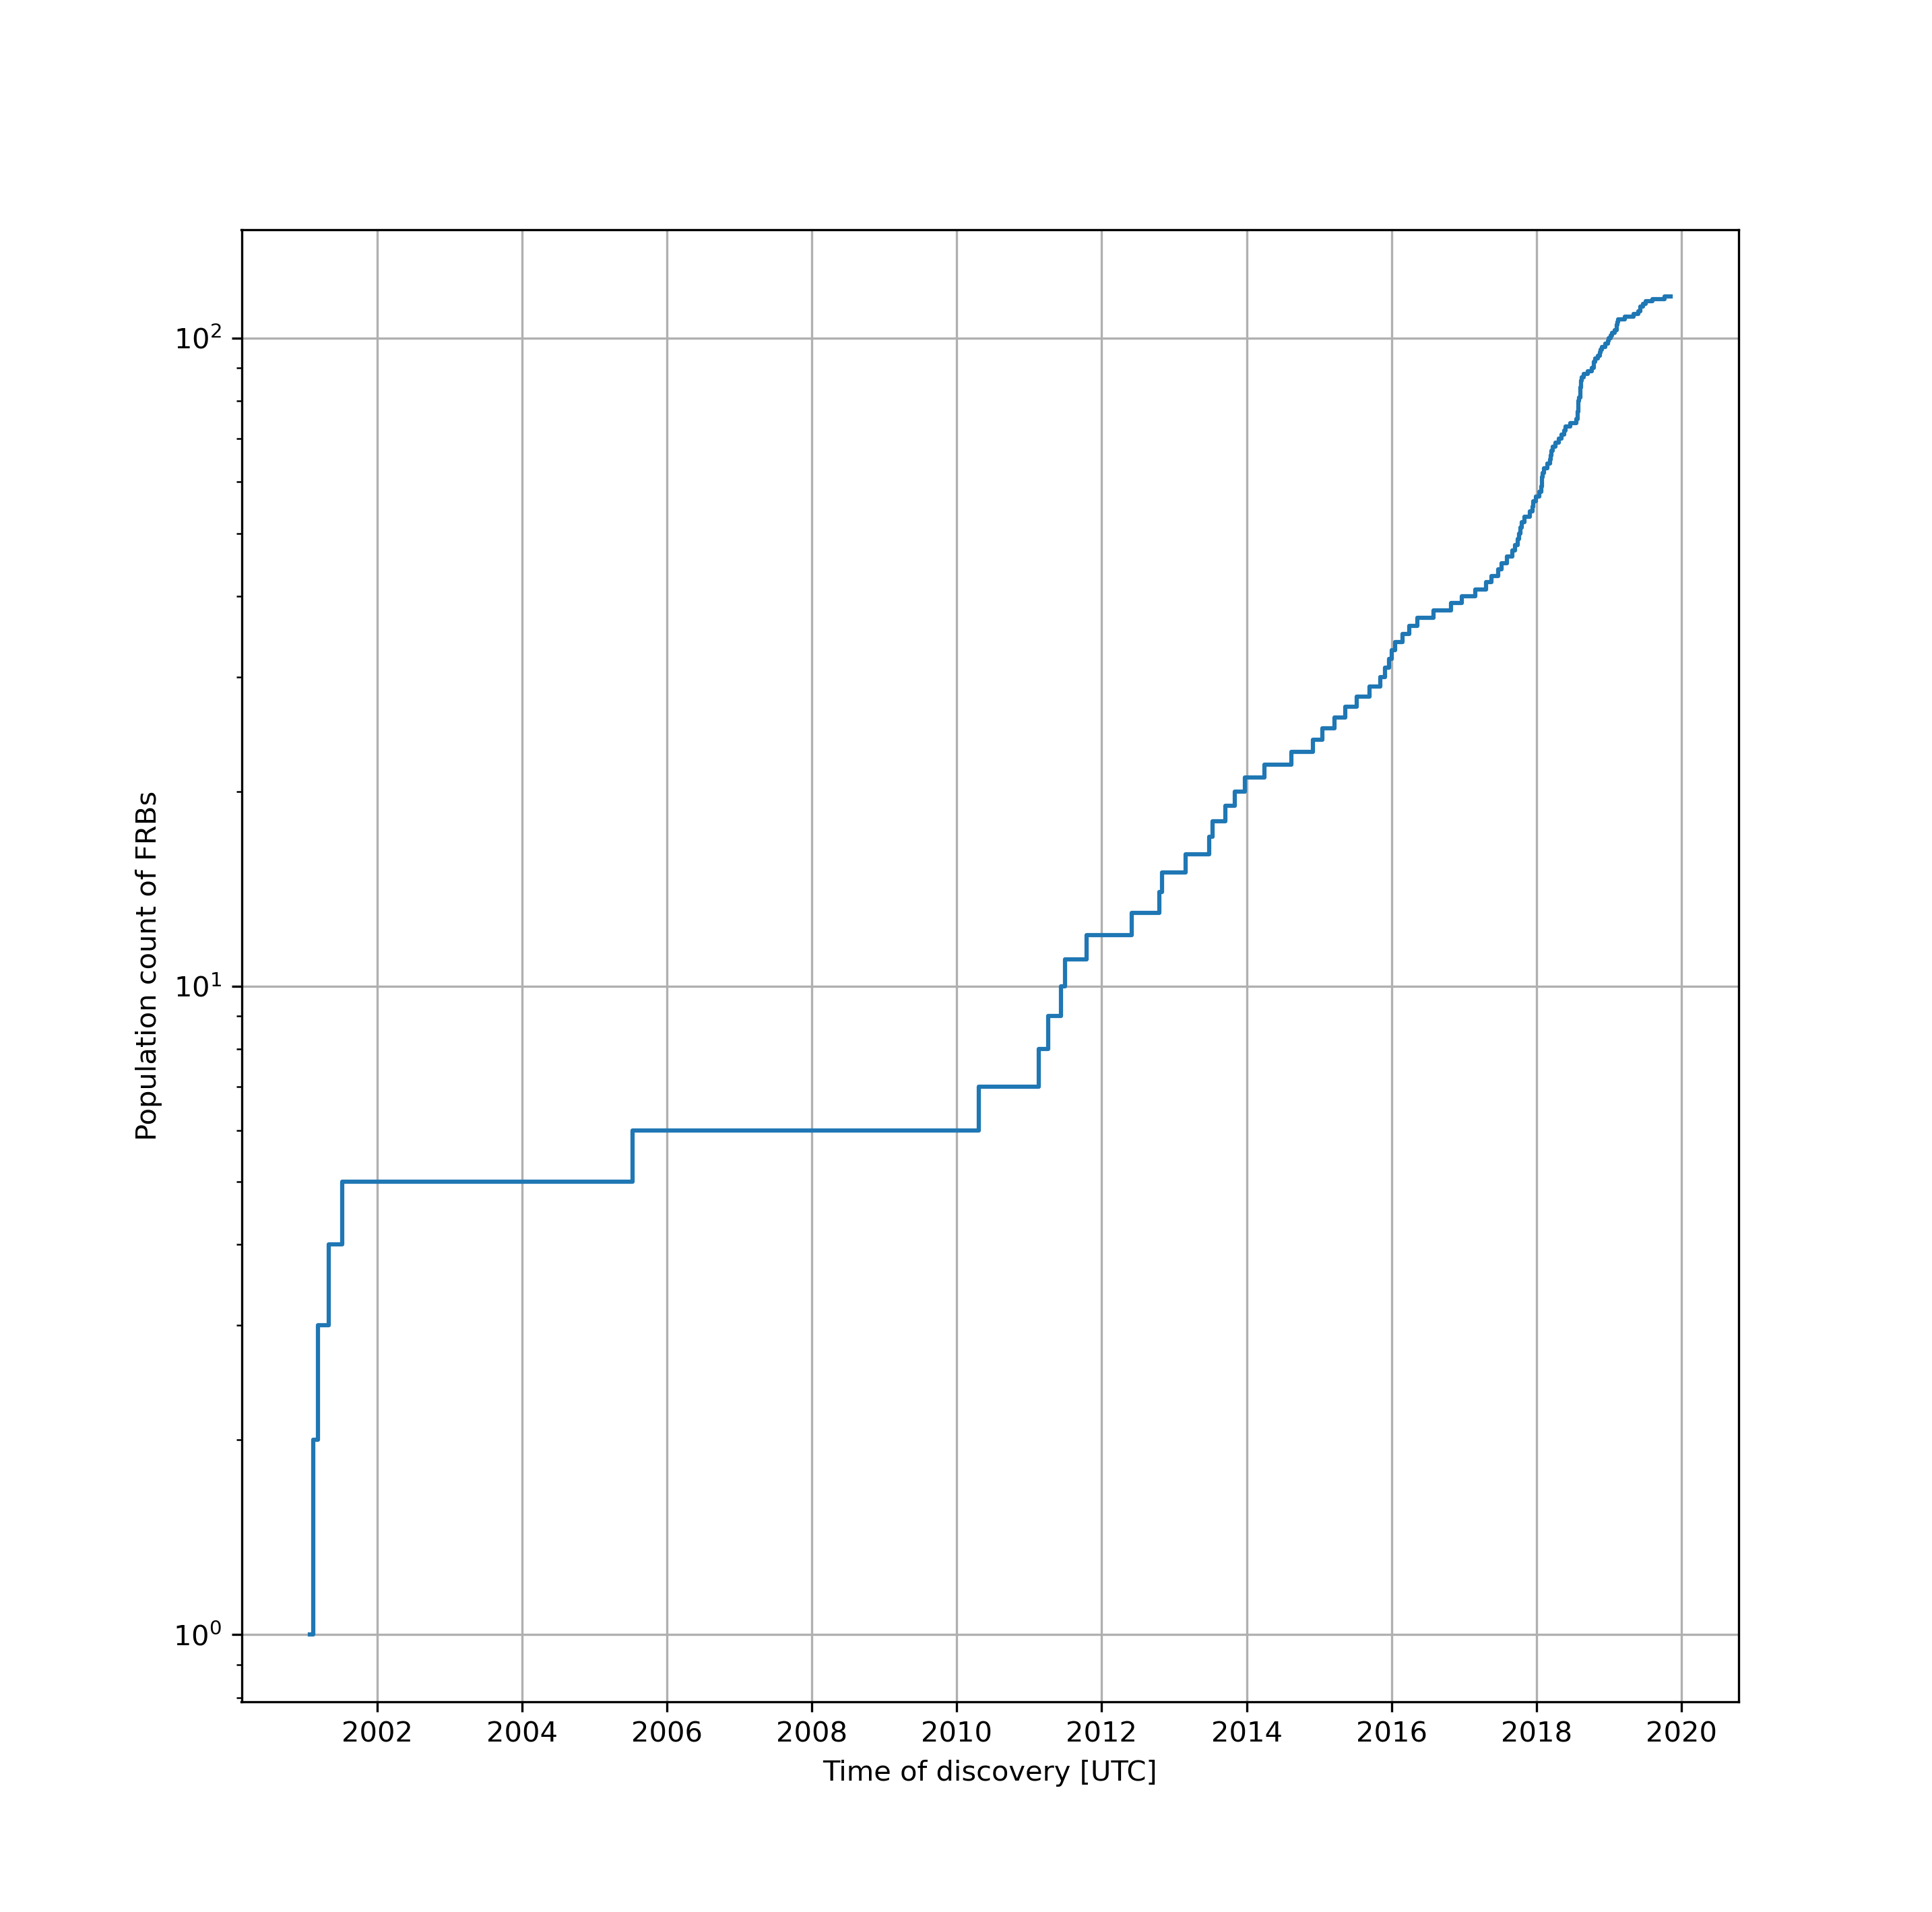
\includegraphics[width=0.8\textwidth, keepaspectratio]{frb_pop.png}
	\caption{Population of \frb{}s over time. The exponential trend is what drives \vf.}
\end{figure}

\begin{figure}
	\label{fig:frbsky}
	\centering
	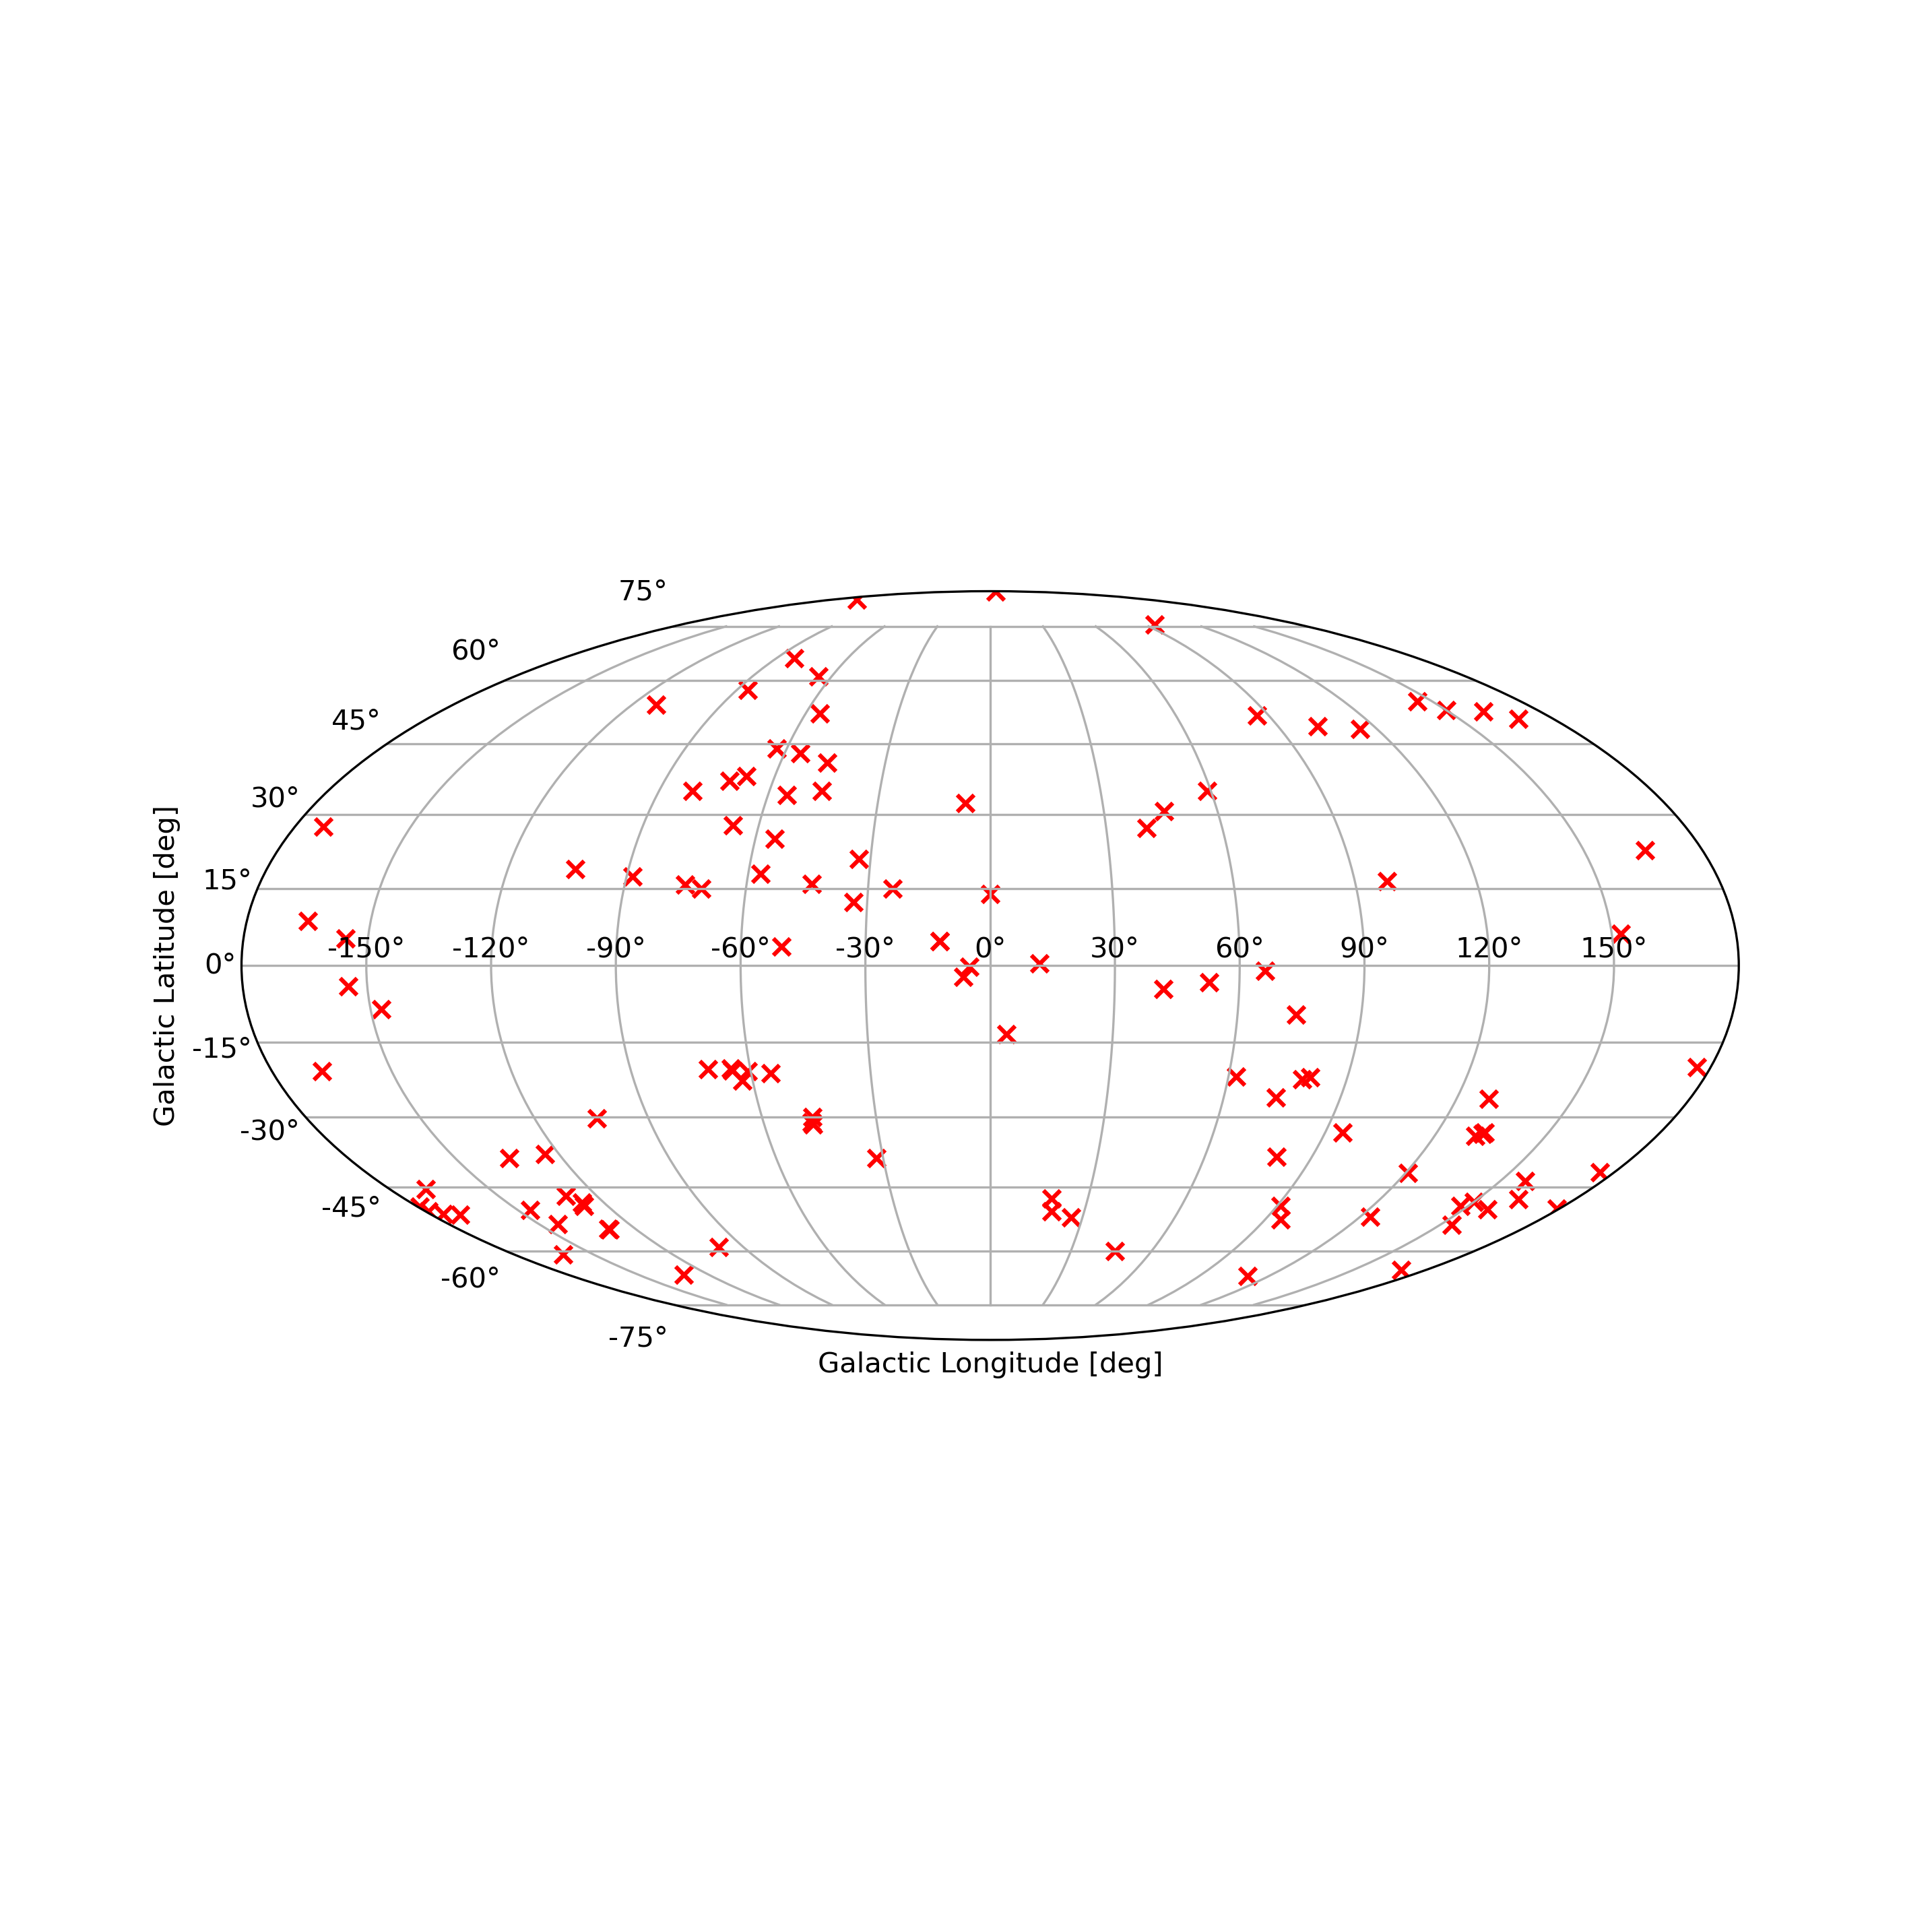
\includegraphics[width=0.8\textwidth, keepaspectratio]{frb_skymap.png}
	\caption{Population of \frb{}s over sky. }
\end{figure}

%\par Lastly, no introduction of \frb{}s is complete without rate calculations. With each survey for these signals, a rate of \frb{}s is computed in the units of per-day-per-sky to quantify the yield of the survey. This metric is rudimentary and shows how much is actually known about them. ~\autoref{tab:frbrates} captures the event rates published by various surveys.

%\begin{table}
	%\label{tab:frbrates}
	%\caption{\frb{}~ event rates with frequency band.}

%\end{table}

\section{Thesis outline}

\subsection{VLITE}

\par This study is a part of the \texttt{VLA Low Frequency Ionospheric and Transient Experiment (\vlite)}. 
\vlite~is a commensual observing system of the Karl G. Janksy Very Large Array radio telescope~(\url{https://science.nrao.edu/facilities/vla}) upon which \vf is based. 
Hence before describing the outline, the \vlite~system is described here.

\par A selected subset of \vla~antennas are fitted with low frequency receiver units at the casegrain feed. 
Receivers are tuned to operate in $320-384$ MHz giving a bandwidth of $64$ MHz. Due to the Mobile Users Operating System (MUOS) of the Department of Defense, the higher end of the band receives a lot of Radio Frequency Interference (RFI), as a result, the frequency band is cut off at $361$ MHz. Nevertheless, the voltage data is sampled at $128$ Mhz (the Nyquist frequency of $64$ MHz bandwidth).
\par The sampled data from each of the antenna is multicast on the observatory intranet using the User Datagram Protocol (UDP) in the form of VLBI Data Interchange Format (VDIF) packets. At the time of writing, there are $16$ \vla~antennas participating in \vlite. \vlite~also consists of $12$ compute nodes with one login node which are interconnected by an Infiniband network~\cite{infiniband}. 
Each compute node houses nVIDIA Graphical Processing Units (GPUs) for all the signal processing and also has a $500$ GB Solid State Disk (SSD) installed.

\par This infrastructure is shared by two different pipelines: \vlite-SLOW and \vf. \vlite-SLOW is an imaging pipeline which produces short time skymaps and is not the focus of this thesis. \vf is a search pipeline which searches for \frb{}s.

\subsection{VLITE as an FRB search engine}
\label{ssub:vfrb}
\par \vlite~is a well suited engine to detect \frb{}s. The salient features are summarized here:
\begin{description}
	\item[Commensal] 
		\vlite~being a commensal system has uncontested access to the data from the \vla antennas.
		This leads to extremely large onsky times which are the times actively looking for signals of interest.
	\item[Large field-of-view (FOV)]
		Each \vlite~antenna is a $25-$meter dish with center frequency of $350$ MHz ($0.85$ meters in wavelength). 
		The diffraction limit of each antenna is $\frac{\lambda}{D}$ where $D$ is the diameter of the dish and $\lambda$ is the wavelength.  
		\vlite~ achieves a diffraction limit of $0.034$ radians or $1.94^o$. 
		An $\sim 2^o$ FOV covers a large portion of the sky. 

	\item[Sensitivity]
		\vlite~employs $16$ antennas.
		Use of a large number of antennas helps in reducing the overall background noise and thereby increases the sensitivity of the signal.
	
	\item[Inteferometer]
		An inteferometer is a type of radio telescope with spatially separated antennas. 
		The spatial separation helps produce a delay between any pair of antennas which is then used to triangulate (localize) the source of the signal. 
		\vla~ is an interferometer. And, hence, \vlite~is too.
		Given how far the \frb{}s are originating from, any task of localizing the cause/source of the signal is hindered by the inability to precisely identify the particular pointing in sky from where the signal has originated.
		Here lies the strength of \vlite~.
\end{description}

\par With the help of these features, \vlite~endevors to be a \emph{FRB localizing search engine}. 

\subsection{Outline}

\par The goal of the study is to establish and start a search campaign making use of the commensual observation system \vlite~of the \vla~radio observatory.
With this in mind, a robust yet efficient realtime search pipeline was designed and coded (see~\autoref{ch:inst}).
The data taken became a part of VLITE-Fast Pathfinder Survey (\vfps). The data is discussed in great detail in~\autoref{ch:data}.
A completeness analysis, in which pure random noise was sent through pipeline, is performed to test the noise response of the pipeline. In addition, artificial signals of interest were inserted into the pipeline for testing the pipeline in a controlled environment. 
The data products yielded by \vfps~and the controlled testing have been used to develop an Aritificial Intelligence (AI) which will be covered in~\autoref{ch:ml}.
The resulting AI solution is used to vet through the entire \vfps~dataset to identify any unknown signal missed previously. Results of the AI analysis are also reported in the same chapter. 



% Instrumentation
\chapter{Instrumentation}
\label{ch:inst}

\par This chapter covers in detail the various pieces of hardware/software which make searching for FRBs possible. As with any data processing/search pipeline, the design consists of various components which are intermediated by data buffers. Such a design allows for modular component design wherein every component is assigned to be either producer or consumer depending on its position and makes it simplier. This practise is not novel in that it is knownas the \emph{producer-consumer} model.

\par Firstly, a brief overview of the infrastructure is summarized in 

\subsection {}

\par Firstly, all the components and the data buffers technology are listed and then approached into details in separate subsequent sections.
\begin{description}
\item[PSRDADA] Data buffer technology
\item[Writer]  Baseband data packet capturing and writing
\item[Process Baseband] Baseband data to filterbank data
\item[Coadder] Co-adding filterbank data from all antennas
\item[Heimdall] Search program 
\item[Trigger mechanics] Set of python scripts for various trigger level activities
\item[TriggerHook]   Identifies slice of data and copies it for future analysis
\item[TriggerMaster] Realtime trigger responses
\end{description}

\par \vf is powered by a $12-$ node cluster each powered by $20$ core Intel Xeon with $64$ GB of Random Access Memory (RAM). Each node also houses \textt{nVIDIA} Titan X for signal processing heavylifting.

\section {PSRDADA}
\par The use of an intermediate buffer is ubiqitious in any real time pipeline. In a producer-consumer model, a producer emits data which is to read by the consumer. In a realtime constrained pipeline, the datarates may not be consistent all the time which may lead to consumer waiting for new data (producer is slow), or unable to accept new data (producer is fast).

\par \vf makes use of \dada as an intermediate buffer technology. \dada is built on SYSV shared memory model thus makes use of linux system's kernels and shared memory infrastructure in offering buffering capability. \dada codebase is in written in \cc for linux type machines. \dada is versatile that it can support the following modes:
\begin{itemize}
\item Single producer - Single consumer (SPSC)
\item Single producer - Multiple consumer (SPMC)
\item Multiple producer - Single consumer (MPSC)
\item Multiple producer - Multiple consumer (MPMC)
\end{itemize}
Of them all, \vf makes use of SPSC, SPMC oweing for a simple logic which involves a single producer.

\par \dada can be visualized as an $n$-element ring buffer with each ring holding $b$ bytes of data. In addition to the data elements, \dada also offers header blocks which can be used to store data descriptors and such information is stored in ASCII.

\section {Writer} 
\hfill \emph {code contributed by Dr. Matthew T. Kerr}

\par \vf is a commensually operated search pipeline. Raw baseband voltage data comes in \texttt{VLBI Data Interchange Format (VDIF)} packets over
\texttt{User Datagram Protocol} network sent by observatory level program called \texttt{executor}. The job of writer is to intercept these data packets and write the header and data into \dada buffer.

\par The raw baseband data consists of two-polarizations, $64$MHz bandwidth real sampled at Nyquist sampling rate of $128$MHz. Writer captures these packets, checks for time ordering and writes into \dada buffer. Time integrity check is of paramount importance since all the following components assume a time continuous flow of data. 

\par Incase writer finds that the incoming packets fail the time continuity check, it is designed to zero fill the packets in between so at least data is continuous in time. The causes for such are many. Sometimes, the ethernet link quality isn't high, or sometimes, the receiving nodes CPU usage is high that it can't respond in time. It has also been observed there are some nodes which are more suspectible to packet drops than other nodes. Such nodes are dropped from subsequent analysis. 

\par Another job of writer is to respond to voltage triggers (see~\autoref{sec:tmech}). For every voltage trigger received, writer writes out one second VDIF file, containing packets, to the Solid State Drive (SSD) onboard for the duration of the trigger. Care is taken that overlapping triggers don't cause duplications of raw voltage files.

\section {Process baseband} 
\hfill \emph {code contributed by Dr. Matthew T. Kerr}

\par Reading raw baseband produced by \texttt{writer}, \texttt{process\_baseband} hereafter, \texttt{pb}, performs the following operations to output filterbank data into another \dada buffer:

\begin{enumerate}
\item Channelization using Fast Fourier Transform (FFT)
\item Polarization addition
\item Bandwidthing and bandwidth normalization
\item Kurtosis filtering
\item Digitization
\end{enumerate}

\par All the above operations are performed on \texttt{nVIDIA} Graphical Processing Units (GPUs). Channelization uses \texttt{CUDA-FFT (cuFFT)}. 
All other operations involve user kernel launches. Addition of polarization yields Stokes \texttt{I} intesity. The upper edge of the \vf frequency band is polluted by the Mobile Users Operation System (MUOS), hence, the maximum frequency is cut off at $360$MHz bringing the effective bandwidth to $42$MHz. 

\par For a large chunk ($\sim 1$s)of data, the bandpass (time averaged frequency profile) is normalized which removes any frequency variations on the time scales of a second. Since, the signals of interest are much smaller in time, such normalization doesn't harm them. In addition to this, there is also a kurtosis based filtering employed which removes any short timescales spurious data.

\par Last operation performed in this component is digitization which digitizes filterbank data with \texttt{NBIT}. Digitization scheme employed follows from~\cite{jenetanderson}. Now, the output data is written to another \dada buffer.

\section {MPI Coadder}

\par Coaddition is the process of averaging time-aligned data streams to produce an averaged data stream. The operation of averaging reduces the noise floor and helps boost the signal.
The motivation for coaddition is firmly established in~\autoref{subs:needcoaddition}. 

\par \autoref{subs:mpic} explains the workings which make coaddition possible in \vf. 
From here on, coadder refers to the component of the \vf which performs coaddition. The underlying technology upon which coaddition operation is based is the Message Passing Interface (\mpi), hence, the coadder is also called \mpi coadder.

\par Coadder reads the filterbank data written to \dada buffer by \pb for all the antennas, coadds, and writes the coadded filterbank data to a \dada buffer residing on a specific node (also called the root node) for further operations. 
In short, the coadder performs, \emph{read-coadd-write} operation in every iteration.

\subsection {Need for coaddition}
\label{ssub:needcoaddition}
\par By the Central Limit Theorem, the distribution of the mean of independent identically distributed (iid) random variables is a Gaussian distribution with mean as the population mean and standard deviation (from here on, \sd) as population \sd divided by $\sqrt{N}$.
The reduction of the \sd means the overall noise has been suppressed to some extent and this proves to be very helpful in any data analysis setting. The extent of the attentuation of noise is determined by the sample size.

\par In addition to the noise suppression, coaddition also helps in bringing out the weaker signal since such a signal would be present in all the antennas, thus would constructively interact and average out to some non zero level. The noise, however, being random around zero level would average out to null.

\subsection {MPI}
\par Message Passing Interface (\mpi) is a technology ubiqitiously used in almost all High Performance Computing (HPC) settings. 
\mpi offers various paradigms heavily optimized for parallized jobs. One such paradigm and also the foundational element is the collective algorithm. 
\mpi defines a collective algorithm as one in which all the processes have to participate as a collection, hence the name collective algorithm. Of all the collective algorithms, only two are used in \vf and discussed here:
\begin{description}
	\item[Broadcast] One process has data which it needs to send to every other process.
	\item[Reduce] All processes have data which is to be combined by some operator and the result is to be made available to a process.
\end{description}
In addition to the above collectives (parlance uesd by the HPC community), there is also the barrier operation which is used to synchronize processes. 

\par The broadcast operation is performed when one process has data (or message) which is sent to all the other processes. At the end of this operation, all processes have identical data. The reduction operation is performed when all processes have some data which is to combined (or reduced) by some operation. The reduced data is present in a pre-defined process called the \root process. 
The process of coaddition is explained in~\autoref{ssub:coadd}. 

\par \mpi also offers capability of tuning by the Multi Component Architecture (MCA). MCA helps you to configure the various runtime parameters of \mpi jobs from pre-defined options to increase the performance. The tuning options used are described in~\autoref{ssub:tuning}.

\subsection {Coaddition}
\label{ssub:coadd}

\par The operation of coaddition involves summation of the data from all the participating processes followed by a scaling. Naturally, the reduce operation with summation operator is a perfect fit for the summation step. 
The scaling operation can then be performed locally. 
The data is read from \dada buffer (which is written to by \pb). This data has been digitized to \nbit by \pb. 
The first operation of coaddition is to convert the \nbit data into \float data. 
This operation increases the memory footprint by four folds but prevents any overflows in reduce operation and is necessary. 
Next comes the actual \mpi reduce call after which, the coadded filterbank data (in \float) is present in \root process.
The resultant \float is then re-digitized to \nbit and written to a \dada buffer present only on the \root node.

\par Before any reduction is performed, it is paramount to check if all the data are time-aligned. 
This time alignment is checked by the \mjd timestamp of the first datum in the array. 
The \root's timestamp is broadcasted to all the other processes which is then compared against the process's own \mjd timestamp. 
If both the \mjd's match, actual filterbank data is used for reduction otherwise a zero-filled array with the same size as the actual filterbank data is used.

\par The scaling operation done after the \mpi reduce call requires the correct number of antennas which have participated in the collective with real data and not with zero data. 
This is computed by another \mpi reduce operation which is done on a single integer set to $1$ if the process is participating with real data, otherwise set to $0$. This operation reduces the actual number of antennas which have contributed for the coaddition.

\par Coaddition is the major bottleneck of the pipeline and it is also the most computationally expensive step. 
A typical gulp of the data is $8$ seconds which with a typical \nchan{4096}, \nbit{8}, and sampling time amounts to $40$ MB.
Due to the casting to \float, the gulp memory footprint shoots up to $160$ MB.
For a typical number of antennas of $15$, every iteration of coaddition involves $160$ MB of floats summed across $15$ antennas, 
making the total bandwidth of the operation to $160\ {\rm MB} \times 15 = 2.4$ GB.
Naturally, the performance of the pipeline depends on the optimizations of the \mpi operations.
Two of the major optimizations are discussed in the following sub-sections.

\subsection {Reduce}
\label{ssub:reduce}

\par Reduction step is the heart of the coaddition. 
Any sort of delay in the coaddition would hurt the realtime operations of the coaddition. 
Consequently, choice of reduction algorithm was delibrated upon.
The following is heavily relied on the seminal paper~\cite{raben}.

\par The default \mpi algorithm for reduce is the binomial tree reduction. 
In this, every 
The entire process is graphically depicted in~\autoref{fig:binreduce}.

\begin{figure}
	\label{fig:binreduce}
	\caption{Binomial algorithm for \mpi reduce of large messages~\cite{raben}.}
\end{figure}

\par Rabenseifner algorithm~\cite{raben} is an alternate reduce algorithm which is well suited for large messages.
Here, every process instead of reducing the entire message is only responsible for reducing a chunk of the message.
After which, all the processes send their reduced chunk back to root.
The entire process is visualized in~\autoref{fig:rabenreduce}.

\begin{figure}
	\label{fig:rabenreduce}
	\caption{Rabenseifner algorithm for \mpi reduce of large messages~\cite{raben}.}
\end{figure}


\par In order to compare different reduction algorithms, a suitable metric has to be introduced.
Metric used in~\cite{raben} is used here. The metric consists of total number of messages sent and total number of bytes sent.
The metric used here is the same in the seminal paper~\cite{raben}.

\begin{figure}
	\label{fig:reducelinear}
	\caption{The linear trend in \texttt{reduce\_coadd} as number of iteration increases.}
\end{figure}

\par The binomial reduce operation uses less messages but the total number of bytes sent is large.

\begin{table}
	\label{tab:reducemetric}
	\caption{Metric for comparing the different reduce operations. c.f. with~\cite{raben}.}
\end{table}

\subsection{Bookkeeping}
\label{ssub:bcast}

% TODO

\par The broadcast of \mjd is a crucial book keeping step. 

\par In the \texttt{Reduce\_numant} step which computes the number of antennas which have participated in the coaddition,
it was observed that occasionally the the time required would shoot to impossibly large times causing pipeline failure.

\begin{figure}
	\label{fig:tcpreduce}
	\caption{Drastically large times for a single value \mpi reduce call zeroed onto the underlying Byte Transfer Layer (BTL) of the \mpi stack being \texttt{TCP}.}
\end{figure}




\section {Heimdall}

\par The search program employed by \vf is Heimdall(~\cite{heimdall}). 
Heimdall is a Graphical Processing Unit (GPU) based search program which performs multiple de-dispersion trials and tophat matched filtering to identify dispersed signals in the data.
GPUs are needed de-dispersion is extremely computationally intensive operation. 
Heimdall internally uses \texttt{dedisp} (~\cite{dedisp}) for de-dispersion.
Tophat matched filtering helps to boost signals. Lastly, normalization of the time series prior to searching regularizes the data.
A simplified algorithm is written in~\autoref{algo:heimdall}. 
Heimdall in reality is much more sophisticated and performs channel masking, and Radio Frequency Interference (RFI) excision. Interested readers are encouraged to read~\cite{heimdall}.

\par Heimdall reads from the \dada~buffer to which coadder writes the coadded data stream. 
It reads a gulp size of data at a time (a parameter optimized, set to $24$ seconds) and performs multiple
\dm-width trials, if the peaks in the resulting de-dispersed, matched-filtered time series data is significant and over a threshold, 
a candidate is registered at that particular \dm~,width, and epoch.
Heimdall sends out these candidates over to Python server running on the login node from where it is suitably acted upon (discussed in the following sections). 
Additionally, Heimdall also writes out the candidates to a candidate file. See~\autoref{ssub:candfile}.

\begin{algorithm}
	\label{algo:heimdall}
	\foreach dm in {2..1000} \do
		\foreach iwid in {1..6} \do
			 de\_disperse (dm) ->
			 matched\_filter ($2^{\rm iwid}$) ->
			 normalize ->
			 search
		\endfor
	\endfor
\end{algorithm}



\section {Trigger mechanics}
\label{sec:tmech}

\par Trigger is a terminology used to denote a candidate which qualifies certain selection rules and warrants follow up action. Trigger mechanics involve receiving triggers from Heimdall, applying selection logic, and performing follow up logic. 
There are two types of triggers: 
\begin{enumerate}
	\item Voltage trigger
	\item DBSON trigger
\end{enumerate}
Voltage trigger, as the name implies, triggers raw baseband voltage data. And, \dbson trigger generates a \dbson file for every trigger. The course of action varies depending on the type of trigger. 
\dbson trigger is treated as the default. If a candidate is to be triggered, then it will \emph{always} have a \dbson trigger.
Each trigger has its own distinct multicast group which makes distinction and follow up action simple and well separated.

\par The underlying \struct which is passed around is the same for both the triggers. \autoref{struct:trigger} shows the struct definition. 
\begin{table}
	\begin{tabular}{llll}
			Index & Name       & Type          & Comments                                               \\
			1     & i0         & double        & UTC start epoch of signal                              \\
			2     & i1         & double        & UTC end   epoch of signal                              \\
			3     & sn         & float         & Signal to Noise ratio of the signal                    \\
			4     & dm         & float         & Dispersion Measure of the signal                       \\
			5     & wd         & float         & Width of the signals in seconds                        \\
			6     & peak\_time & float         & Time since UTC epoch start of signal when signal peaks \\
			7     & meta       & char{[}128{]} & Meta information                                      
	\end{tabular}
	\caption {Trigger struct definition. Signal here means the signal of interest. See text for more information.}
	\label{struct:trigger}
\end{table}

\par Voltage trigger handling is solely performed by the writer (see~\autoref{sec:writer}). \dbson trigger response is much more sophisticated and will be dealt in the following sub-sections.

\subsection {Trigger dispatch}

\par Heimdall in addition to writing candidate files, also sends candidate data over to server which is called the trigger dispatch. 
The purpose of trigger dispatch is to receive candidates, apply various candidate selection logics, and multicasts triggers over to the compute nodes. 
Trigger dispatch is written purely in Python.

\par Each selection rule consists of cuts on \sn, \dm, and \wd. In practise, multiple rules are used simultaneously. Moreover, special notch filters to target pulses from pulsars are also applied. 
The type of selection rules used and the triggers received are discussed in great detail in \autoref{ch:data}. Hence, only a simple example of a rule is provided here:
\begin{align*}
	{\rm S/N} &\geq 8 \\
	{\rm DM} &\geq 50 {\rm\ pc/cc} \\
	{\rm Width} &\leq 100 {\rm\ ms}
\end{align*}

\par By default, trigger dispatch only sends out \dbson triggers. More stringent set of rules is applied in case of voltage triggers. 
The reason being SSD space required for voltages is much much more than that required for \dbson~s. 
A typical rule for a \dbson trigger to also be a voltage trigger is a simple cut as, \sn $\geq 25$. Such a simple rule allows for any serendiptious voltage triggering on strong triggers.

\subsubsection {Throttling}
\label{sssub:rfim}
\par Dispatching all the triggers received may sometimes overload the pipeline, cause lags, and may ultimately fail the pipeline.
Hence, a suitable trigger throttling mechanism is put in place.
Trigger rate may skyrocket for a multitude of reasons. It may be so whenever a bright radio pulsar in in the field-of-view (FOV) of \vf.
It may also be when Radio Frequency Interference (RFI) is strong, causing a large number of spurious triggers.
Given the frequency band of operation ($320|384$ MHz) being not just close to walky-talkies used by on-site engineers but also being close to MUOS band, \vf~is more suspectible to RFI.
Presence and effects of RFI is discussed more in detail in~\autoref{sec:RFI}. 
Here, only the instrumentation part of the throttling is described.

\par Heimdall performs searches in batches. All the candidates from a batch are sent at once after the batch has been processed.
Throttling is done at a sub-batch level. A typical batch size is $30720$ samples ($\sim 24$ seconds) and the sub-batch is $8$ seconds.
Using the metrics defined and discussed in~\autoref{sec:RFI}, a sub-batch is vetted and subsequently dispatched.
Throttling is performed on a sub-batch and not on a batch level since a batch lasts long, doing over a sub-batch offers finer control and instanteneous response.
Moreover, $8$ is also the dispersion delay for the highest \dm~ searched for.

\subsection {Trigger hook}

\par Any type of follow-up analysis requires the filterbank data spanning for the duration of the trigger. The job of Trigger hook is to receive the \dbson trigger, slice the appropriate filterbank data, and write it along with trigger information into \dada buffers.

\par Input to trigger hook is the same \dada buffer used by Heimdall for its searching. Output of trigger hook are two separate \dada buffers, one for trigger information (header) and one for trigger data (data). 
\dada offers header block in a buffer but the number of headers is hardcoded to $8$ which would severly reduce the number of triggers that can be held in buffer to $8$.  Hence, two separate buffers are employed.

\par Trigger Hook reads the buffer and keeps track of the UTC epochs of the first sample in each data-block as it reads. 
Then, for a trigger received, with some pointer arithmetic, a slice of filterbank data is written to the data \dada buffer and trigger information is written to header \dada buffer.

\par Trigger hook also holds the option to write out a \fbson. But, this option is not typically used since follow up action is performed anyway.

\subsection {Trigger master}

\par Reading from the buffer to which Trigger Hook has written the sliced filterbank along with trigger information, Trigger master performs the following:
\begin{itemize}
	\item Generating: 
		\begin{itemize}
			\item De-dispersed filterbank binary JSON (\dbson, see~\autoref{ssub:dbson})
			\item Trigger plot (see~\autoref{ssub:tp})
		\end{itemize}
	\item Machine learning (ML) based classification of the trigger and baseband triggering.
\end{itemize}

\par The following only discuss the generation of \dbson~and trigger plot. 
The entirity of classification is discussed in great detail in~\autoref{chap:ml}.
Firstly, the bowtie plane is introduced. And

\par The bowtie plane is computed using the Fast De-dispersion Measure Technique (FDMT,~\cite{fdmt}).
The low frequency introduces large delays which make the FDMT algorithm extremely slow. 
Hence, prior to FDMT, the data is first incoherently de-dispersed to first \dm and then FDMT is applied.

\begin{figure}
	\label{fig:bt}
	\caption{Bowtie plane. \sn as a function of \dm and time. 
	It is called a bowtie plane since a true dispersed signal produces a bowtie.
	Insets are the frequency averaged integrated profiles at different \dm~s.
}
\end{figure}

\begin{figure}
	\label{fig:dd}
	\caption{Left: Dispersed filterbank. Right: De-dispersed filterbank.}
\end{figure}

\subsection {Meta response}
\par For every voltage trigger issued, a variety of meta data has to be packaged to do any kind of analysis with the voltage data. 
This job is performed by Meta response. Meta data involves the following:
\begin{enumerate}
\item Antenna mappings
\item Antenna delays
\item Antenna positions
\item Trigger parameters
\end{enumerate}

\par This job is done by a Python server running on the login node. 
This server listens to the mcast group to which voltage triggers are issued.
For a voltage trigger, it outputs a \textt{metar} file as described in~\autoref{ssub:metar,tab:metar}.

\section {Data products}
\par This section defines all the data products of the pipeline. 
\subsection {Candidate file}
\label{ssub:candfile}
\par A candidate file consists of tab-separated values. Every new line has either two fields or nine fields. 
The definition of the file is given in~\autoref{tab:candfile}.
% Please add the following required packages to your document preamble:
% \usepackage{multirow}
\begin{table}[]
	\label{tab:candfile}
	\caption{Description of candidate file.}
	\begin{tabular}{lll}
		\begin{tabular}[c]{@{}l@{}}Type of\\ data\end{tabular} & \begin{tabular}[c]{@{}l@{}}Number of\\ fields\end{tabular} & Data                                                                                                                 \\
		\multirow{2}{*}{Pointing}                              & \multirow{2}{*}{2}                                         & Right Ascension in radians                                                                                           \\
																													 &                                                            & Declination in radians                                                                                               \\
		\multirow{9}{*}{Candidate}                             & \multirow{9}{*}{9}                                         & Signal to Noise ratio of the candidate                                                                               \\
																													 &                                                            & \begin{tabular}[c]{@{}l@{}}Index of the first sample of the signal since\\ the start of the observation\end{tabular} \\
																																																									&                                                            & Time of the first sample of signal                                                                                   \\
																																																									&                                                            & Filterwidth of the signal                                                                                            \\
																																																									&                                                            & Index of the DM trial                                                                                                \\
																																																									&                                                            & DM of the signal                                                                                                     \\
																																																									&                                                            & Number of giants in the group                                                                                        \\
																																																									&                                                            & UTC epoch of the start of the signal                                                                                 \\
																																																									&                                                            & UTC epoch of the end of the signal                                                                                  
										 
 \end{tabular}
\end{table}
\begin{table}
	\label{tab:ubson}
	% Please add the following required packages to your document preamble:
	% \usepackage{multirow}
	\begin{tabular}{llll}
		\hline
		Type                        & Parameter   & Present & Comments                                               \\ \hline
																& S/N         & Both    & Signal to Noise ratio of the trigger                   \\
																& DM          & Both    & Dispersion Measure of the trigger                      \\
																& Width       & Both    & Width of the trigger in seconds                        \\
		\multirow{4}{*}{Time}       & Peak time   & Both    & Peak time of the trigger from the start of the data    \\
																	& Tstart      & Both    & MJD of the start of the data                           \\
																	& Tsamp       & Both    & Sampling time of the data                              \\
																	& Duration    & Both    & Duration of the data                                   \\
		\multirow{3}{*}{Frequency}  & Fch1        & Both    & Frequency of the first channel in MHz                  \\
																	& Foff        & Both    & Frequency width in MHz                                 \\
																	& Nchans      & Both    & Number of channels in the data                         \\
		\multirow{4}{*}{Indices}    & I0          & Both    & UTC epoch of the first sample of the data              \\
																	& I1          & Both    & UTC epoch of the last sample of the data               \\
																	& Epoch       & Both    & UTC epoch of the start of the observation              \\
																	& Nsamps      & Both    & Size of the data                                       \\
		\multirow{6}{*}{Parameters} & Nbits       & Both    & Number of bits per datum                               \\
																	& Antenna     & Both    & Station ID                                             \\
																	& Source name & Both    & Name of the source observing when trigger was recorded \\
																	& RA          & Both    & Right Ascension of the source in radians               \\
																	& Dec         & Both    & Declination of the source in radians                   \\
																	& Group       & Both    & String identifier                                      \\
		DMs                         & DM1         & DBSON   & Start DM in pc/cc in bowtie plane                      \\
																& DMoff       & DBSON   & DM width in bowtie plane                               \\
																& NDM         & DBSON   & Number of DM trials in bowtie plane                    \\
		Data                        & FB          & FBSON   & Raw filterbank                                         \\
																& DD          & DBSON   & De-dispersed filterbank                                \\
																& BT          & DBSON   & Bow-tie plane                                          \\ \hline
	\end{tabular}
\end{table}
\subsection {FilterBank jSON}
\par FilterBank jSON (\fbson) is an Universal Binary JSON~\cite{ubjson} file format containing unprocessed filterbank along with header information. Filterbank data is in time major format with frequency index changing the fastest.
The schema is defined in~\autoref{tab:ubson}. 
\par This data product is no longer in use since the trigger processing is currently done in realtime.
\subsection {De-dispersed filterBank jSON}
\label{ssub:dbson}
\par De-dispersed filterbank jSON (\dbson) is an Universal Binary JSON~\cite{ubjson} containing de-dispersed filterbank and bowtie plane digitized to \uchar.
The schema is defined in~\autoref{tab:ubson}.
\subsection {Trigger plot}
\label{ssub:tp}
\par Trigger plot is a diagnostic plot generated for every trigger. 
It is saved in Portable Networks Graphics (PNG,~\cite{png}) format and rendered used PGPLOT~\cite{pgplot} library.

\par A trigger plot consists of bow-tie plane, de-dispersed filterbank, frequency averaged time profile, and \dm profile. 
In addition to them, a trigger plot also shows \sn, width, pointing information, and time information.
A typical trigger plot for a known pulsar trigger is given in~\autoref{fig:tp}.

\begin{figure}
	\label{fig:tp}
	\caption{A trigger plot generated on a trigger realtime. This trigger is from a pulsar.}
\end{figure}

\subsection {META Voltages}
\label{ssub:metar}
\par Meta (\meta) is an Universal Binary JSON~\cite{ubjson} containing meta information required for any voltage analysis.
% Please add the following required packages to your document preamble:
% \usepackage{multirow}
\begin{table}[]
	\label{tab:metar}
	\caption{Schema for Meta dumped for every voltage trigger.}
	\begin{tabular}{lll} \toprule
		Type                     & Parameter      & Comments                                                                                                               \\ \midrule
		\multirow{5}{*}{Header}  & S/N            & Signal to Noise ratio of the trigger                                                                                   \\
														 & DM             & Dispersion Measure in pc/cc of the trigger                                                                             \\
														 & Width          & Width of the trigger in seconds                                                                                        \\
														 & T0             & UTC epoch of the start of the signal                                                                                   \\
														 & T1             & UTC epoch of the end of the signal                                                                                     \\
		\multirow{8}{*}{Delays}  & VLITE\_ANT\_ID & VLITE Antenna ID                                                                                                       \\
														 & VLA Antenna    & VLA Antenna                                                                                                            \\
														 & DIFX\_HOST     & Compute node connected to the antenna                                                                                  \\
														 & DIFX\_IFACE    & Network interface on the compute node                                                                                  \\
														 & CLK\_OFFSET    & Clock offset in nanoseconds                                                                                            \\
														 & PAD            & Antenna string identifier                                                                                              \\
														 & LO\_FIBER      & RF-over-Fiber delay in nanoseconds                                                                                     \\
														 & ENABLE         & If antenna is added to the array                                                                                       \\
		\multirow{7}{*}{Antprop} & CONFIG         & Array configuration identifier                                                                                         \\
														 & DATASETID      & Dataset identifier                                                                                                     \\
														 & CREATION       & Epoch of creation                                                                                                      \\
														 & EOPSET         & \begin{tabular}[c]{@{}l@{}}Earth Orientation Parameter set.\\ TAI\_UTC, UT1\_UTC and \\ pole information.\end{tabular} \\
																																																				& dots           & For each EOPDAY                                                                                                        \\
																																																				& ANTS           & \begin{tabular}[c]{@{}l@{}}Antenna information.\\ WIDAR\_ID, PAD, X, Y, Z, OFFSET\end{tabular}                         \\
																																																																													& dots           & For each antenna                                                                                                      
																																																																								\bottomrule
	\end{tabular}
\end{table}

% Data taking
% Data analysis
\chapter{VLITE-Fast Pathfinder Survey}
\label{ch:data}

\par This chapter summaries the entirity of the data collected in numerous runs of the \vf system, and follows it up careful statistical analysis. All triggers from known sources are summarized.


\section {Campaign runs}

\par \vfpfs consists of data collected over multiple settings. 
Any campaign run is characterized by the type of filterbank data used and the kind of trigger cuts used. This characterization breaks the whole of \vfpfs into multiple fragments. Each fragment is summarized separately in the respective sub-sections. 

\par Firstly, all the campaign runs are enumerated and discussed in brief before delving into the details in respective sub-sections.
\begin{description}
	\item[NBIT = 2 (NB2)] \\
		This was the first run of \vfpfs system. All the filterbank data was set to $2$ bits to test the computational capabilities of the pipeline. Conservative trigger cuts were employed for the same reason.
	\item[NBIT = 8 (NB8)] \\
		The filterbank data bit depth was increased to $8$ in this run. The trigger cuts were the same as before.
	\item[Max Warp (MW)] \\
		The trigger cuts were drastically changed to the most aggressive possible. 
\end{description}

The key features are summarized in ~\autoref{tab:campaigns}.

\begin{table}
	\caption{Salient features of all the campaign rules involved in \vfpfs.}
	\label{tab:campaigns}
\end{table}

\subsection {NB2}

\par In an epoch from \texttt{2019-10-17} to \texttt{2019-12-05} spanning for $49$ days, \vf was onsky for $27.05$ days. 
This resulted in capturing $10\ 573$ triggers, yielding a trigger rate of $13\ {\rm hr}^{-1}$. The uptime achieved in this was $55.2\%$.

\par The main features of this run was that the data was digitized to \nbit{2} hence the name. Moreover, this was the pilot run for the \vf system.
The trigger cuts were as follows:

\par This run didn't have the \dbson trigger mechanics in place. Instead, for every trigger \fbson~ files were written to disks at all the antennas including the coadded antenna as well.

\subsection {NB8}

\par In an epoch from from \texttt{2019-12-10} to \texttt{2020-01-20}spanning $40$ days, \vf was onsky for $16.67$ days.

\subsection {MW}


\section {Detection of pulsars}

\par A large onsky time yields many serendiptious triggers caused by pulses from pulsars. 
These detections are a field test for \vf and diagnostic information can be derived from it. 
Based on these detections, a rudimentary argument for Field of View (FOV) (~\autoref{ssub:fov}) and sensitivity (~\autoref{ssub:sensitiviy})is formulated.


\begin{table}
\caption {Observed pulsars}
\end{table}

\subsection{Field of View}
\label{ssub:fov}

\par It is worthwhile to understand the spatial extent over which the \psr{J1752} (from now on dm50) has been detected. 
This exercise would help us understand how large of a field-of-view \vf posses.
See ~\autoref{fig:dm50fov}. 
\begin{figure}
	\label{fig:dm50fov}
	\caption{Large FOV of \vf understood using \psr{J1752} as a marker. 
	Dots represent the pointings where triggers from the pulsars were recorded.
	Numbers next to the dots represent fraction of the total number of triggers detected at the pointing.
}
\end{figure}

\subsection {Sensitivity}
\label{ssub:sensitiviy}

\par The sensitivity of the \vf~ can be understood using the detected set of pulsars.
Since, each pulsar has a documented flux density at $400$ MHz, available in \texttt{PSRCAT}(~\cite{psrcat}).
With the help of number of pulses detected, the sensitivity of \vf~ can be loosely extrapolated on the basis of the pulsars.

\begin{figure}
	\label{fig:psrs400}
	\caption{Sensitivity of \vf using triggers from pulsars and documented flux density. 
		Flux density is plotted on x-axis. Triggers received divided by time spent on sky is plotted on the y-axis.

}
\end{figure}
\section {RFI}
\label{sec:RFI}

\par One of the major challenges any radio observatory faces is that of Radio Frequency Interference (RFI). 
These are spurious radio signals of human origin polluting the frequency band of interest. In a search pipeline such as \vf, 
RFI causes large number of triggers which tax the pipeline. 
One of the main reasons for \vf pipeline failing from time to time is the lag caused by serving many spurious triggers because of RFI.
Naturally, with the triggers collected so far, a strategy can be devised to understand the triggers caused by RFI and mitigate them realtime.
This is described in~\autoref{ssub:rfim}. \vfpfs also observed recurring RFI which produces a distinct feature in the \dm~ distribution. This artifact is discussed in~\autoref{ssub:dm150}.

\subsection {RFI mitigation}
\label{ssub:rfim}

\subsection {\DM{150} artifact}
\label{ssub:dm150}

\par Short time RFI in a single frequency channel does not produce spurious triggers since bandpass normalization on the time windown containing the RFI cancels its intensity. 
However, when there is short time RFI in separate channels, it is a different story. 
If such a short time RFI is coincident in time, any search pipeline would register it as a \DM{0} signal and can be filtered out easily.
But, if the same RFI has a time offset between the frequency channels, it causes the same search pipeline to register spurious triggers and are much more difficult to excise.

\par In a short time RFI only exisiting in specific frequency channels having time offset between the channels, behaves like a dispersed signal. And when the filterbank is de-dispersed for that \dm which aligns the short time RFI, the excess power causes triggers. 

\par The same is observed in \vfpfs which causes triggers at a range of \dm~s centered around \DM{150}, hence the name. See the de-dispersed filterbank and frequency averaged profile in~\autoref{fig:rfidm150}.

\begin{figure}
	\label{fig:rfidm150}
	\caption{}
\end{figure}

\section {Heimdall triband structure}
\par A complete statistical analysis of all the triggers also uncovered the extent of capability of Heimdall in its \dm-width trials.
See~\autoref{fig:triheimdall} which is expected to be uniform in the \dm-width parameter space. 
However, for large \dm~s, Heimdall employs a time averaging window (known as tscrunching) which reduces the sensitivity in the width. 
This is captured by the quantization seen in the width space for large \dm.

\par Heimdall performs the tscrunching operation by default. 
This operation is a feature of the underlying de-dispersion code called \textt{dedisp}(~\cite{dedisp}) which is used by Heimdall. 
For large \dm, the in-channel smearing (introduced in~\autoref{sssub:dd}) is very high and at times exceeds the sampling time. In such a case, time averaging is performed which increases the sampling rate and the in-channel smearing is kept less than the sampling time.
If the in channel smearing is much more than the sampling time, the signal is lost. Any amount of de-dispersion would not bring out the signal.

\par In all the runs so far, the \texttt{adaptive\_dt} was enabled. 
An effect of this feature is that for weak \sn, large \dm signals if the width is not near any of the quantized widths, the matched filtering would not boost the signal causing it to be passed as non-detection.

\par An artifact of this is seen in excess triggers registered at specific \dm~s beyond which tscrunching is performed prior to searching.
These \dm~s are found to be \DM{347.165} and \DM{790.695} for which the in-channel smearings at highest, lowest and central frequencies are tabulated at~\autoref{tab:dmsmearing}.

\begin{table}
	\label{tab:dmsmearing}
	\caption{In-channel smearing at \dm~s where tscrunching is activated for the lowest and highest frequency channels. The sampling time is $781.25\ \mu$s and frequency channel width is $655.255$kHz.}
	% Please add the following required packages to your document preamble:
	% \usepackage{multirow}
		\begin{tabular}{llll}
			DM (pc/cc)               & Frequency (Mhz) & Smearing (ms) & Time units \\
			\multirow{3}{*}{347.165} & 361.941         & 19.9          & 25         \\
															 & 340.973         & 23.8          & 30         \\
															 & 320             & 28.8          & 36         \\
			\multirow{3}{*}{790.695} & 361.941         & 45.3          & 58         \\
															 & 340.973         & 54.2          & 69         \\
															 & 320             & 65.6          & 84        
		\end{tabular}
\end{table}

\begin{figure}
	\label{fig:triheimdall}
	\caption{\dm-Width space of all the Heimdall triggers. Although the maximum width is set to $100$ ms, this plot only extends until $20$ ms.
		This space is expected to be uniform.
	}
\end{figure}

\begin{figure}
	\label{fig:histdm}
	\caption{Histogram of \dm of all the triggers recorded.}
\end{figure}


\section{Summary statistics}
\par total uptime, sky coverage, number of candidates
\par that distribution



% ML/AI
\chapter{Machine Learnings}
\label{ch:ml}

\par This chapter describes the Machine Learning (ML) / Artificial Intelligence (AI) system in the \vf which identifies triggers worthy of a closer look. First and foremost, the motivation is discussed in~\autoref{sec:coh}.
The ML model is introduced and described in~\autoref{sec:ml}. 
Lastly, the newly \emph{learnt} ML model is applied to the whole of \vfpfs and results are examined in~\autoref{sec:ml_vfps}.

\section {Coherent analysis}
\label{sec:coh}

\par \vf operates on an \emph{incoherent} level. In all of the pipeline, only the power is considered.
There is no phase considered anywhere. This lack of phase greatly simplifies the pipeline design but comes at a cost.
Hence the name, \emph{incoherent}.

\par For an array of $N$ antennas, co-addition in \emph{incoherent} (see~\autoref{ssub:needcoaddition}) only boosts the signal (or specifically, the signal-to-noise, \sn) by $\sqrt{N}$. 
An \emph{coherent} analysis would boost the \sn~by $N$.

\par In addition to the \sn~boost, a \emph{coherent} analysis would also provide good localization capability.
This localization ability is of great value since \frb~s are known to be originating from outside the galaxy by which small angular variations could lead to astronomically large separated distances due to large radii.

\subsection{Coherent analysis with \vf}

\par In order to be able to do \emph{coherent} analysis, voltage data has to be recorded. 
A second of raw voltage data consisting of two polarization measures about $250$ MB. 
A typical \vf compute node has $450$ GB of dedicated Solid State Disk (SSD). Meaning, a \vf compute can only have $1800$ s (or $30$ minutes) of raw voltage data before getting filled.
Given the extremely large volume of voltage data, it is impractical to record voltages all the time.
Hence, \vf performs searches \emph{incoherently} and triggers voltages for a coherent follow-up analysis.

\par It is also not practical to trigger voltages on all the triggers. It would be so as if voltages are recorded all the time since the trigger rates are high.
So only a subset of the triggers received are to be allowed to trigger voltages. 
Naturally, such a subset has to be selected on the basis of the signal's merit of being a real signal of astrophysical origin.
The question of how to decide what triggers to trigger on is the main goal of this chapter.

\section {ML models}
\label{sec:ml}


\section {Applying ML to VFPS}
\label{sec:ml_vfps}

\par Having the newly \emph{learnt} set of AI models, a retrospect analysis of all the triggers part of \vfpfs is performed to uncover any previously missed triggers.
Results are 



% This makes the bibliography.
% Enter your references in the BibTex file "references.bib"
% You can find bibtex info from Google Scholar.
\bibliographystyle{siam}
\bibliography{references}


% Uncomment the \appendix macro below for appendices
% Insert appendix chapters after the macro
%\appendix


% This inserts your Biographical Sketch
\biographypage

\end{document}
